\section*{Ergebnisse}
\label{sec:Ergebnisse}

Das Kaiser-Meyer-Olkin-Kriterium der Faktorenanalyse nimmt für die betrachteten Variablen aus dem "`Insel"' Datensatz einen Wert von 0,734 an.
Das entspricht einem ziemlich guten Maß an Interkorrelation zwischen den Variablen \cite{eckey2002multivariate}, womit sie sich für eine Faktorenanalyse eignen.
Entsprechend dem Kaiser-Kriterium für signifikante Faktoren ab einem Eigenwert von mindestens 1, erstellt die Faktorenanalyse aus den 13 Variablen vier Faktoren.
Die vier Faktoren erklären insgesamt 67\,\% der Gesamtvarianz.
Wenige Variablen laden dabei relativ stark in einen Faktor, während sie gleichzeitig eher schwach in die übrigen Faktoren laden.
Einzig die Variable \textit{Emotional} lädt in keinen der Faktoren stark und wird aus diesem Grund für die inhaltliche Beschreibung der erzeugten Faktoren nicht berücksichtigt.
Die vier erzeugten Faktoren werden inhaltlich gekennzeichnet als $Ruhig_f$ für den 1. Faktor, $Niveauvoll_f$ für den 2. Faktor, $Heiter_f$ für den 3. Faktor und $Energisch_f$ für den 4. Faktor (vgl. Tabelle \ref{tab:faktoren}).   


\begin{table}[htbp]
    \centering
    \caption{Ergebnis der Faktorenanlyse mit den jeweiligen Faktorladungen.}
    \vspace{3mm}
    \label{tab:faktoren}
        \begin{tabularx}{8.4cm}{|lY|r|lY|}
            \multicolumn{2}{c}{1. Faktor: \textbf{Ruhig}} & \multicolumn{1}{c}{} & \multicolumn{2}{c}{2. Faktor: \textbf{Niveauvoll}} \\
            \cline{1-2}\cline{4-5}
            ~Entspannend & ~0,821~     &  & ~Anspruchsvoll & ~0,862~ \\
            \cline{1-2}\cline{4-5}
            ~Warm & ~0,811             &  & ~Komplex & ~0,736 \\
            \cline{1-2}\cline{4-5}
            ~Sanft & ~0,777            & &  ~Einfach & -0,701 \\
            \cline{1-2}\cline{4-5}
            \multicolumn{2}{c}{}       & & ~Intellektuell & ~0,669 \\
            \cline{4-5}
            \multicolumn{5}{c}{} \\
            \multicolumn{2}{c}{3. Faktor: \textbf{Heiter}} & \multicolumn{1}{c}{} & \multicolumn{2}{c}{4. Faktor: \textbf{Energisch}} \\
            \cline{1-2}\cline{4-5}
            ~Fröhlich & ~0,855          &   & ~Erregend & ~0,838 \\
            \cline{1-2}\cline{4-5}
            ~Traurig & -0,713           &  & ~Intensiv & ~0,656 \\
            \cline{1-2}\cline{4-5}
            ~Tanzbar & ~0,680           & \multicolumn{1}{c}{} & \multicolumn{2}{c}{} \\
            \cline{1-2}
        \end{tabularx}
\end{table}


Die Regressionen der ermittelten Faktoren mit den Features von Spotify liefern Modelle mit sehr guten Signifikanzen nahe 0 (vgl. Tabelle \ref{tab:regression}).
Als Kriterium für das Aufnehmen einer Variable in ein Modell darf maximal ein Signikanzwert von 0,05 erreicht werden.  
Das Modell mit der höchsten Güte erhalten wir bei der Regression mit dem Faktor $Heiter_f$.
23,1\,\% der Varianz wird vom Modell mit den Variablen \textit{danceability}, \textit{energy}, \textit{instrumentalness} und \textit{valence} gedeckt.
Die Variable \textit{energy} ist in dem Modell am stärksten gewichtet, gefolgt von den Variablen \textit{danceability},  \textit{instrumentalness} und \textit{valence}.
Das Streudiagramm dieses Modells ist in Abb. \ref{fig:Faktor3} zu sehen.    
Ein Modell mit einem ähnlich hohem Bestimmtheitsmaß $R^2$ gibt die Regression mit dem Faktor $Ruhig_f$ aus, die 21,5\,\% der Varianz deckt.
Enthalten in diesem Modell ist die Variable \textit{energy}, die mit einer negativen Effektstärke etwa vier mal stärker gewichtet ist als die zweite in dem Modell enthaltenen Variable \textit{speechiness}.
Deutlich schlechtere Modellanpassungen liefern die Regressionen mit den Faktoren $Niveauvoll_f$ und $Energisch_f$.
Wir erhalten ein Modell mit einer Güte von 0,112 bei der Regression mit dem Faktor $Energisch_f$ und nur 0,038 bei der Regression mit dem Faktor $Niveauvoll_f$.

\begin{table}[htbp]
    \centering
    \caption{Ergebnisse der Regressionen aus SPSS}
    \vspace{2mm}
    \label{tab:regression}
        \begin{tabularx}{8,4cm}{@{\extracolsep{\fill}} @{\arrayrulewidth1.5pt\vline}c@{\arrayrulewidth1.5pt\vline}X|c|c|l@{\arrayrulewidth1.5pt\vline}}
            \noalign{\hrule height1.5pt}
            \textbf{Faktor} & \textbf{Modell} & \textbf{Beta} & \textbf{Sig.} & \textbf{$R^2$} \\
            \noalign{\hrule height1.5pt}
            \multirow{2}{*}{Ruhig}  & ~energy & -0,434 & 0,000 & \multirow{2}{*}{0,215~} \\
                \cline{2-4}
                & ~speechiness & -0,100 & 0,040 & \\
            \noalign{\hrule height1.5pt}
            \multirow{2}{*}{Niveauvoll} & ~instrumentalness & ~0,130 & 0,020 & \multirow{2}{*}{0,038} \\
                \cline{2-4}
                & ~loudness & -0,110 & 0,048 & \\
                \noalign{\hrule height1.5pt}
            \multirow{4}{*}{Heiter} & ~danceability & ~0,247 & 0,000 & \multirow{4}{*}{0,231} \\
                \cline{2-4}
                & ~energy & ~0,279 &  0,000 & \\
                \cline{2-4}
                & ~instrumentalness & ~0,204 & 0,000 & \\
                \cline{2-4}
                & ~valennce & ~0,136 & 0,021 & \\
                \noalign{\hrule height1.5pt}
            \multirow{3}{*}{Energisch} & ~valence & -0,238 & 0,000 & \multirow{3}{*}{0,112} \\
                \cline{2-4}
                & ~loudness & ~0,287 & 0,000 & \\
                \cline{2-4}
                & ~instrumentalness & ~0,139 & 0,010 & \\
            \noalign{\hrule height1.5pt}
        \end{tabularx}
\end{table}

\begin{figure}[hbt]
    \begin{center}
        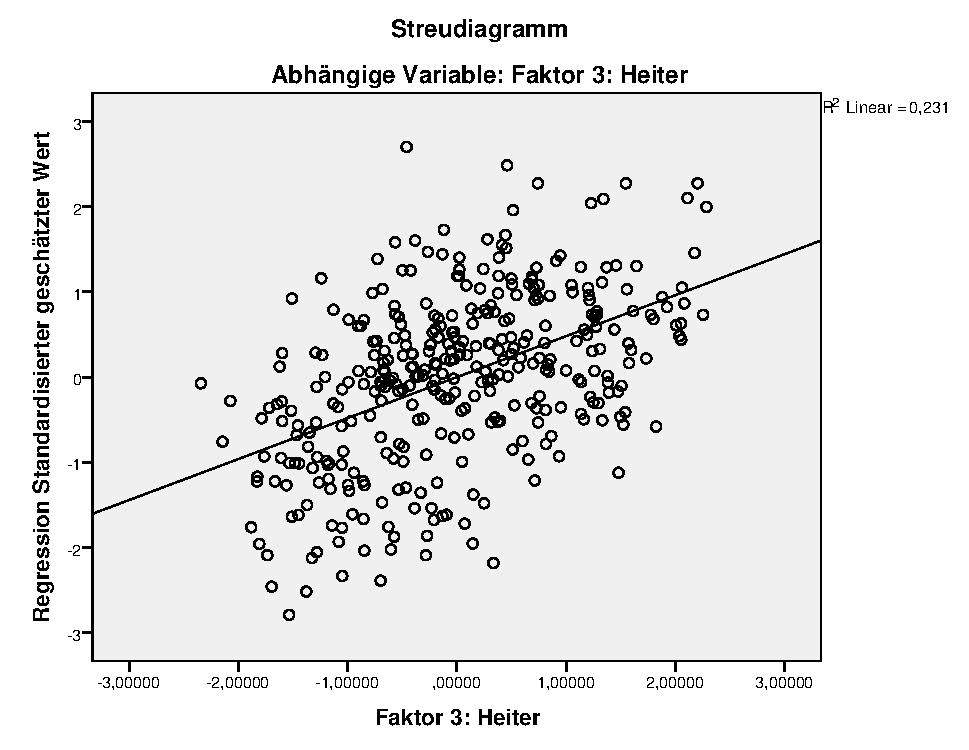
\includegraphics[width=8cm]{images/StreudiagrammFak3.pdf}
    \end{center}
    \caption{Streudiagramm und Regressionsgerade der Regression mit dem Faktor $Heiter_f$. Diese liefert die beste Modellanpassung.}
    \label{fig:Faktor3}
\end{figure}

\section*{Diskussion}
\label{sec:Diskussion}


Die Modelle der Regressionen sind hochsignifikant.
Somit ist ein Zusammenhang zwischen den Bewertungen der Probanden und den Features von Spotify vorhanden.
Die Effektstärken der Modelle sind dagegen eher gering. 
Während die Regressionen mit den Faktoren $Heiter_f$ und $Ruhig_f$ mit Korrelationskoeffizienten von 0,481 und 0,464 nah an den in der Hypothese formulierten Wert kommen, liegen die Korrelationskoeffizienten für die Regressionen mit den Faktoren  $Energisch_f$ (0,335) und vor allem $Niveauvoll_f$ (0,195) deutlich darunter.
Die Deutung der Korrelationswerte der erstellten Modelle deckt sich auch mit der Interpretation von Effektstärken von Cohen \cite{cohen1988}.
Dabei entspricht der Korrelationswert $r$ für die Regression mit dem Faktor $Niveauvoll_f$ einem kleinen Effekt, die übrigen entsprechen immerhin einem mittleren Effekt.
Ein starker Effekt, der bei einem Korrelationswert von mindestens 0,5 vorzufinden ist, wird nicht erreicht.
Somit kann die in der Hypothese formulierte Annahme einer starken Korrelation der Datensätze mit einem Wert von mindestens 0,5 nicht bestätigt werden. 

Die Ergebnisse zeigen, dass die MIR Verfahren von Spotify zur Bewertung von Musikstücken noch Verbesserungspotential haben.
Jedoch sind auch beim Datensatz "`10 Songs für die einsame Insel"' Fehler zu erwarten, die in einen kleineren Korrelationskoeffizienten resultieren könnten.
Die Songs wurden jeweils nur einmal von einer einzelnen Person bewertet.
Hinzu kommt, dass die Probanden einen besonderen, persönlichen Bezug zu den von ihnen bewerteten Musikstücken haben.
Eine höhere Anzahl an Bewertungen eines einzelnen Musikstücks durch mehrere Probanden mit anschließender Mittelung würden die in diesem Datensatz vorhandenen Fehler minimieren.

Ein weiterer Grund für die geringe Korrelation könnte die inhaltlich meist nicht direkt entsprechenden Bewertungskriterien beider Datensätze sein.
Es gibt beispielsweise für den Faktor mit dem schwächsten Korrelationswert ($Niveauvoll_f$) kein Spotify Feature, das diesem Faktor inhaltlich zugeordnet werden kann.
Dahingegen lässt sich eine starke negative Korrelation des Spotify Features \textit{energy} mit dem Faktor $Ruhig_f$ inhaltlich sinnvoll erschließen.
Gleiches gilt auch für die Korrelation der Features \textit{danceability}, \textit{energy}, \textit{instrumentalness} und \textit{valence} mit dem Faktor $Heiter_f$.
Jedoch wurde eine größere Abhängigkeit dieser inhaltlich ähnlichen Variablen, vor allem \textit{danceability} und \textit{valence}, mit dem Faktor $Heiter_f$, erwartet.
Die Spotify Features \textit{tempo}, \textit{liveness} sowie \textit{acousticness} korrelieren dagegen nicht signifikant mit einem der Faktoren und werden in keinem Modell aufgenommen. 
Das Audio Feature \textit{tempo} beschreibt eher die Struktur eines Musikstücks, ähnlich wie die schon im Vorhinein von der Analyse nicht berücksichtigten Audio Features (\textit{duration\_ms}, \textit{time\_signature} und \textit{key}).
Daher ähnelt das Feature \textit{tempo} auch inhaltlich keinem der subjektiver Empfindungen entsprechenden Bewertungen aus dem "`Insel"' Datensatz.
Die Audio Features \textit{liveness} und \textit{acousticness} entsprechen inhaltlich ebenfalls keinem der "`Insel"'-Variablen.  

Mit einer neuen empirischen Studie, bei der die in dem Datensatz "`10 Songs für die einsame Insel"' vorzufindenden Bewertungskriterien für Musikstücke konkret durch die Audio Features von Spotify ersetzt werden, kann an die in diesem Paper gewonnenen Forschungsergebnisse angeknüpft werden.



